\chapter{Firmware Verification and Validation}
\label{chapter:vv}
This chapter contains the documentation of testing and verifying the quality of the released firmware. 
\section{Testing Methodology}
This section describes how the firmware testing is setup and executed. 
\subsection{Testing Strategy}
The firmware is tested based on the following testing strategies and methods: 
\begin{itemize}
 \item \textbf{Positive Testing}: Verification of the unit tests is based on expected results from valid input value(s).
 \item \textbf{White Box Testing}: the unit tests are written by developers who looked up the source code and made the test cases based on this. 
 \item \textbf{Ad Hoc Testing}: for the purpose of development speed and rapid-prototyping, tests are performed on based on intuition and on-the-fly cases/scenarios. 
 \item \textbf{Compatibility Testing}: the compilation of the firmware and the unit test is compile-able on various hardware devices types. Like Windows, Linux, Mac OS and ARM. 
 \item \textbf{Mock Testing}: Due to strong dependency with hardware modules, like I2C mocks were needed to simulate(mock) the signals or functionality of the real objects.
\end{itemize}
\subsection{Test Environment}
The testing environment is setup and configured in VS code IDE. The testing framework is Google Testing library, which is used for software test suites (combination of test cases) and mocks for hardware interfaces.\\\\
Testing of the sensor functionality (not validation of the reading result, outside of the project scope) is done by connection with the hub and analyzing the stream data. 
\subsection{Test Coverage Goal}
The most essential system components are tested. Essential components are the data aggregation transducers, because the main function of the system is to gather the data reliably.
\section{Code Examples}
To give an ideal of how the unit test are written, there are a couple of examples with description.\\
\begin{figure}[h!]
  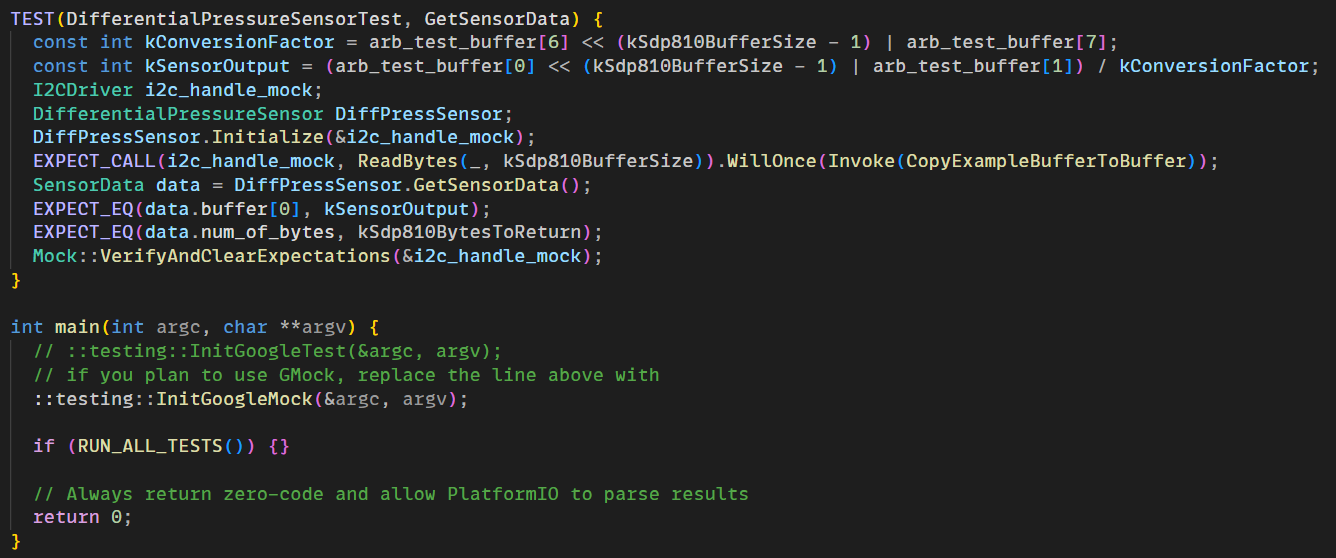
\includegraphics[scale=0.60]{figures/Code example.png}
  \caption{Unit testcase example}
\end{figure}\\
The test case is named "DifferentialPressureSensorTest" and specifically test the "GetSensorData" function that it inherited from the abstraction class "Universal Sensor".\\
Here is a short explanation of what the test case does:
\begin{enumerate}
    \item The test case defines a constant variable "kConversionFactor" based on values from the "arb\_test\_buffer" array. This variable is used in calculating the expected sensor output.
    \item The test case creates an instance of the "I2CDriver" class which is a mock called: "i2c\_handle\_mock" and an instance of the "DifferentialPressureSensor" class called "DiffPressSensor".
    \item The "Initialize" function of the DifferentialPressureSensor is called with the "i2c\_handle\_mock" instance.
    \item An expectation is set on the "ReadBytes" function of "i2c\_handle\_mock" to read "kSdp810BufferSize" number of bytes and invoke the "CopyExampleBufferToBuffer" function.
    \item The "GetSensorData" function of "DiffPressSensor" is called, and the returned value is stored in the "data" variable of type "SensorData".
    \item Two expectations are set to check the correctness of the sensor data:
        The first expectation uses "EXPECT\_EQ" to check if the first byte of "data.buffer" is equal to the calculated "kSensorOutput".\\
        The second expectation checks if the "num\_of\_bytes" member of "data" is equal to "kSdp810BytesToReturn".
    \item Finally, the "VerifyAndClearExpectations" function is called on the "i2c\_handle\_mock" instance to verify that the expectations were met and clear them for subsequent tests.
\end{enumerate}
Overall, this test case initializes a mock I2C driver, sets expectations for reading specific bytes, calls the "GetSensorData" function, and checks if the received sensor data matches the expected values. This is an example that comes out of the current state-of-art firmware version. Other test cases and suites are really similar to this example.\\\\ 
\section{Test Results}
\begin{table}[]
\begin{tabular}{|l|l|l|l|l|l|}
\hline
Test ID & Test case & Expected Out & Actual Out & Result & Comment \\ \hline
1 & Compression Sensor &  &  & PASS &  \\ \hline
1.1 & initialize() & \begin{tabular}[c]{@{}l@{}}Function calls of \\ I2C driver, write commands\end{tabular} & Right calls of I2C driver. & PASS &  \\ \hline
1.2 & GetSensorData() & 0xAF & 0xAF & PASS &  \\ \hline
2 & \begin{tabular}[c]{@{}l@{}}Differential \\ Pressure Sensor\end{tabular} &  &  & PASS &  \\ \hline
2.1 & initialize() & \begin{tabular}[c]{@{}l@{}}Function calls of \\ I2C driver, write commands\end{tabular} & Right calls of I2C driver. & PASS &  \\ \hline
2.2 & GetSensorData() & 6 & 6 & PASS &  \\ \hline
3 & Finger Position Sensor &  &  & PASS &  \\ \hline
3.1 & initialize() & \begin{tabular}[c]{@{}l@{}}Function calls of \\ I2C driver, write commands\end{tabular} & Right calls of I2C driver. & PASS &  \\ \hline
3.2 & GetSensorData() & \begin{tabular}[c]{@{}l@{}}0x05, 0x00, 0x85, 0x99, \\ 0x91, 0x74, 0x55, 0x14\end{tabular} & \begin{tabular}[c]{@{}l@{}}0x05, 0x00, 0x85, 0x99, \\ 0x91, 0x74, 0x55, 0x14\end{tabular} & PASS &  \\ \hline
\end{tabular}
\end{table}